\documentclass[twocolumn,11pt]{IEEEtran}
\usepackage{epsfig}
\usepackage{amssymb}
\usepackage{amsmath}
 
%-----------------------

\begin{document}


\title{SecureIM a encrypted chat client}


\author{Arne Bjune and Vegar Engen \\ \texttt{\{arnedab,vegaen\}@cs.ucsb.edu}}

\markboth{SecureIM a encrypted chat client}{Bjune and Engen}

\maketitle

\begin{abstract}
With the recent scandals in government mass surveillance the need for a secure way to communicate becomes clear for anyone that wants to keep their communication private. With this application we aim to use private-public
 keys cryptography to secure the communication between android users. \end{abstract}

\section {Introduction}
\label{sec:introduction}
For this project we wanted to implempent an instant messaging clint for android. We called the application Secure IM. The purpose of the application is that you should be able to send messages to your friends without having to worry about that other people are reading your messages. To do that we have implemented an application that uses RSA encryption to when sending messages. One of the biggest issues by using applications to send messages secure is that you have to trust the developer or the server provided by the developers, and because of that reason our project is a open-source and are availabe at http://www.github.com/vegaen/SecureIM. It includes the server and the client, so the users are free to set up their own server if do not put enough trust in the server provided. 


In this paper we are going to cover our design for a secure chat client that uses a combination of symmetric AES encryption and RSA public key encryption. Software design choices will be covered inn section \ref{sec:design}, the authentication protocol in section \ref{sec:auth} and possible improvements in section \ref{sec:improve}. 


\section {Software Design}
\label{sec:design}
This application has a server-client architecture, where the android-devices are clients and needs a server to run. All messages goes through the server. If the server receives a message that is for another user it redirects it to the right reciever.

The application are built for Android 4.2.2 with the android sdk 17. It consists of one Activity that uses fragments to display the different screens, and running different Threads and Asynctasks for servercommunication. It opens into a login screen where the user is prompt for username. If a private RSA-key does not exist locally for the user it is creates a Key Pair. The authentification process is more discussed in section \ref{sec:auth}. When a user want to connect to another user, it askes the server if that person is available. If it is the application opens a chat view and makes it possible for the user write a message. The message is being encrypted at the client and sent to the server, which redirects it to the user you want to contact. When you receive a messsage it is decrypted with your private key and is viewed on the screen.



\section{Authentication Protocol}
\label{sec:auth}
To authenticate the users the server sends a randomly generated challenge the user signs with its private key. This first message is the only message sent in cleartext, the rest is encrypted. Along with the authentication challenge the server supplies its public key, the clients compares it with its stored key, if the clients has no key it accepts and stores the supplied key. The signed challenge from the server is sent back with the clients desired username and public key. The server first checks if it has a public key that corresponds to he username supplied by the  If a key is found, the server uses the stored key to verify the signed challenge. If no key is found, the supplied key is used and stored for further use.

After both server and client have been authenticated the client sends a request to connect to another user, if the requested user is logged in the server supplies the corresponding public key and establishes a connection.A message sequence chart for the authentication protocol can bee seen in Figure \ref{fig:auth}. All packets are still pass through the server but the content is encrypted with the client's private keys so the server is not able to decrypt it.


\begin{figure}
\label{fig:auth}
\centerline{
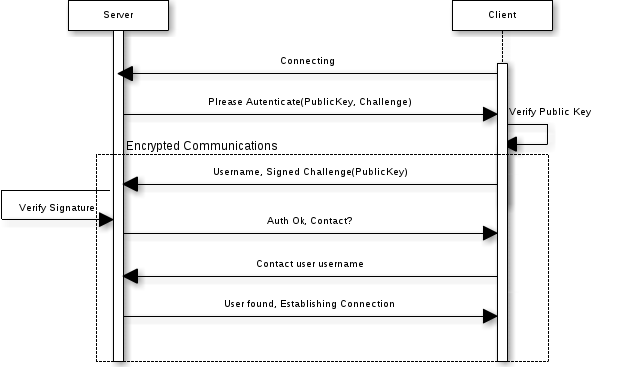
\includegraphics[width=90mm]{auth.png}}
\caption{Authentication process}
\end{figure}

 \section{Crypto}
When a messages passes through the server the to and from fields gets decrypted and the server uses them to know were to forward the packet. Before the packages is forwarded the to and from fields are encrypted with the receiving clients public key.

 Because public key cryptography is an expensive operation we generate a symmetric key for every message that is used to encrypt the message text. The symmetric key is then encrypted with the receiving clients public key. 

\section{Problems}
\label{sec:problems}


\section {Conclusion}
\label{sec:conclusion}
We now have a fully functioning application for sending encrypted messages, there is not a lot of advanced features but it is a good foundation to continue working on. The messages are encrypted and only visible on the clients.

\section {Improvements and future work}
\label{sec:improve}
Currently a message going from one client to another needs 4 public key operations and 

Even if the clients use public key cryptography the server still has to be trusted to deliver the correct keys and not replacing them with its own. This could be improved by transferring the keys directly from one client to another but this brings up a lot of challenges with devices behind firewalls. However since both the server and client and server are open source you could easily run your own server to provide the needed server trust.

Adding a seed when encrypting the to and from fields should also be added to avoid a eavesdropper from gaining information about how many users are contacted and how often. 

%\bibliographystyle{IEEEbib}
%\bibliography{my}


\end{document}
